\documentclass[12pt,onecolumn,a4paper,fleqn]{article}
\usepackage[top=1in, bottom=1in, left=0.75in, right=0.75in]{geometry}
\usepackage{epsfig,graphicx,subfigure,amsthm,amsmath}
\usepackage[table,xcdraw,svgnames]{xcolor}
\usepackage{setspace}
\usepackage{mathtools}
\usepackage{fancyhdr}
\usepackage{sidecap}
\usepackage{tikz}
\usepackage{pgfplots}
\usetikzlibrary{decorations.pathreplacing}
\usepackage{relsize}
\usepackage{color,xcolor}
\usepackage[framed,numbered]{matlab-prettifier}
\usepackage{float}
\usepackage{enumerate}
\usepackage{booktabs}
\usepackage{setspace}
\usepackage{datetime}
\usepackage{xepersian}


\settextfont[Path=fonts/,BoldFont={ZarBd.ttf},BoldFeatures={Scale=0.9}]{BZar.ttf}

%\DeclarePairedDelimiter\ceil{\lceil}{\rceil}
%\DeclarePairedDelimiter\floor{\lfloor}{\rfloor}

\definecolor{vgreen}{RGB}{104,180,104}
\definecolor{vblue}{RGB}{49,49,255}
\definecolor{vorange}{RGB}{255,143,102}

\pagestyle{fancy}
\fancyhf{}
\rhead{\textbf{آزمایشگاه طراحی سیستم‌های دیجیتال}}
\chead{\textbf{گزارش آزمایش پنجم}}
\lhead{\textbf{\nouppercase{\rightmark}}}
\cfoot{({\thepage})}
\renewcommand{\headrulewidth}{1pt}
\renewcommand{\footrulewidth}{1pt}
\renewcommand{\sectionmark}[1]{\markright{#1}}
\renewcommand{\subsectionmark}[1]{\markright{#1}}
%\newdateformat{monthyeardate}{%
%	\monthname[\THEMONTH], \THEYEAR}

\onehalfspacing
\begin{document}
	%%% title pages
	\large
	\begin{titlepage}
		
		\begin{center}
			\begin{huge}
				\textbf{
					به نام خدا\\
				}
			\end{huge}
			
			\vspace*{1.5cm}
			
\includegraphics[scale=0.9]{source/sharif_logo.png}\\
			\vspace*{0.5cm}
			\begin{Large}
				
				دانشگاه صنعتی شریف\\
				\vspace*{0.25cm}
				\textbf{
					دانشکده مهندسی کامپیوتر\\
				}
			\end{Large}
			\vspace*{3cm}
			\begin{huge}
				\textbf{
					آزمایشگاه طراحی سیستم‌های دیجیتال\\
					\vspace*{1.75cm}
				}
			\end{huge}
			
			\begin{Large}
				\textbf{
					آزمایش پنجم:\\
					طراحی واحد ضرب‌کننده\\
				}
			\end{Large}
			
			\noindent\rule[1ex]{\linewidth}{1pt}
			\vspace*{1.5cm}
			\begin{Large}
				محمدجواد هزاره، یاسین موسوی
				
				\vspace*{1.5cm}
				%					\textbf{\today}
				\textbf{
					تابستان 1400
				}
			\end{Large}			
		\end{center}
		\thispagestyle{empty}
	\end{titlepage}	
	\pagebreak
	
	\tableofcontents
	\thispagestyle{empty}
	\pagebreak
	\section{مقدمه}
	\subsection{هدف آزمایش}
	در این آزمایش هدف طراحی یک واحد ضرب‌کننده به روش الگوریتم
	\lr{Booth}
	بود.
	\subsection{مبانی تئوری}
	الگوریتم 
	\lr{Booth}
	یک الگوریتم برای ضرب دو عدد $n$ بیتی در یکدیگر بوده که براساس روش 
	\lr{Add \& Shift}
	است. مراحل این این الگوریتم در شکل \ref{fig:booth-alg} آمده است.
	\begin{figure}[H]
		\centering
		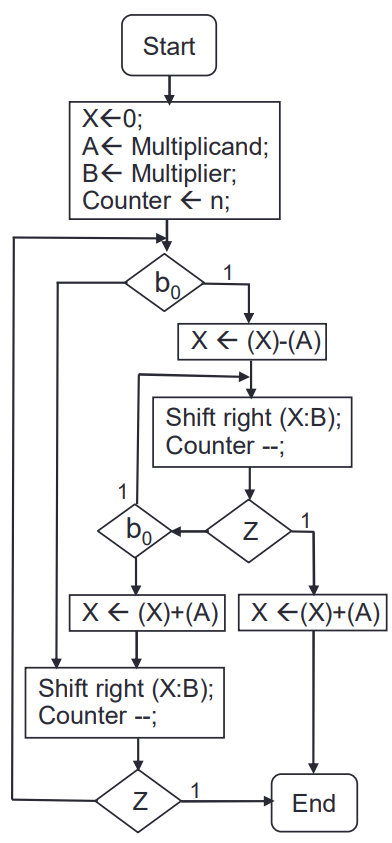
\includegraphics[scale=0.8]{source/booth-alg.png}
		\caption{مراحل الگوریتم \lr{Booth}}
		\label{fig:booth-alg}
	\end{figure}
	\pagebreak
	\section{معماری مدار}
	\subsection{روش کار}
	برای پیاده‌سازی الگوریتمی که در شکل \ref{fig:booth-alg} نشان داده شد، دو واحد مسیر داده و واحد کنترل در نظر می‌گیریم. واحد کنترل در واقع یک ماشین حالت است که حالت‌های مختلفی که در الگوریتم داریم را طی کرده و مسیر داده نیز با توجه به حالتی که این ماشین در آن قرار داد، داده‌ها را جمع و یا تفریق کرده و شیفت می‌دهد.
	\subsection{واحد کنترل}
	همانطور که گفته شد این واحد یک ماشین حالت است که نمودار آن را در شکل \ref{fig:state-graph} می‌توان دید.
	\begin{figure}[H]
		\centering
		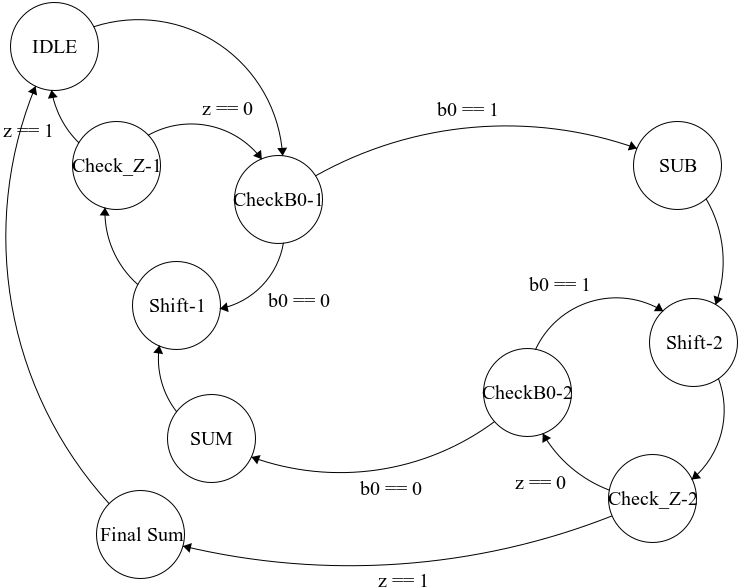
\includegraphics[scale=0.5]{source/finite-state.png}
		\caption{ماشین حالت واحد کنترل}
		\label{fig:state-graph}
	\end{figure}

	با توجه به تقارن نمودار، می‌توان حالت‌هایی که زیروند دارند را با استفاده از یک متغیر دیگر تشخیص داد و برای آن‌ها حالت جدیدی در نظر نگرفت.
	
	ورودی‌های این واحد نیز سیگنال‌های 
	\lr{data\_ready}
	و
	\lr{b0}
	هستند که به‌ترتیب نشان دهنده آماده بودن اعداد و شروع به کار واحد ضرب‌کننده و بیت اول ضرب‌کننده می‌باشند. خروجی‌‌های آن نیز 
	\lr{o\_subtract}
	،
	\lr{o\_result\_ready}
	و
	\lr{o\_state}
	هستند که سیگنال اول نشان‌دهنده نوع عملیات محاسباتی‌‌ای است که باید صورت بگیرد (تفریق یا جمع ضرب شونده) و کاربرد سیگنال‌های دیگر نیز از اسم آن‌ها مشخص است.
	\subsection{مسیر داده}
	این قسمت با استفاده از حالتی که واحد کنترل دارد، تصمیم به جمع یا تفریق ضرب‌شونده با رجیستر کمکی \lr{X} می‌گیرد. ورودی‌های آن اعداد
	\lr{A}
	و
	\lr{B}
	به همراه سیگنال‌های 
	\lr{state}
	و
	\lr{subtract}
	که از واحد کنترل می‌آیند می‌باشد. خروجی‌های آن نیز 
	\lr{b0}
	و
	\lr{result}
	هستند که \lr{b0} در واحد کنترل استفاده شده و \lr{result} نیز جواب ضرب را نشان می‌دهد.
	\pagebreak
	\section{شبیه‌سازی عملکرد مدار}
	در شکل \ref{fig:simulation} شبیه‌سازی مدار برای ضرب اعداد 3 و 13 آورده شده که در آن می‌توان حالت ماشبن واحد کنترل و عملکردی که مسیر داده داشته است را مشاهده کرد.
	\begin{figure}[H]
		\centering
		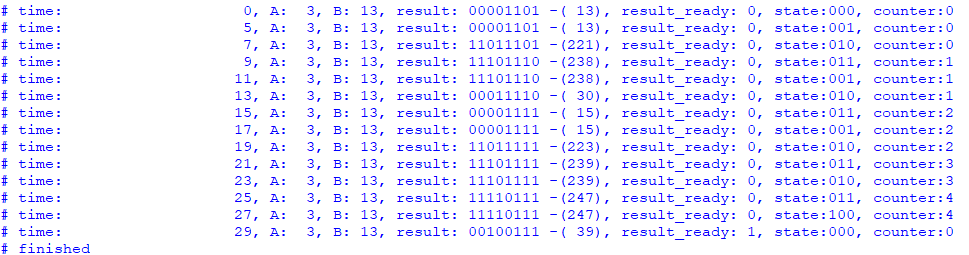
\includegraphics[scale=0.8]{source/simulation.png}
		\caption{ضرب 3 در 13}
		\label{fig:simulation}
	\end{figure}
\end{document}